\chapter{Decision Trees \& 
Influence Diagrams}

\begin{figure}[h!]
\centering
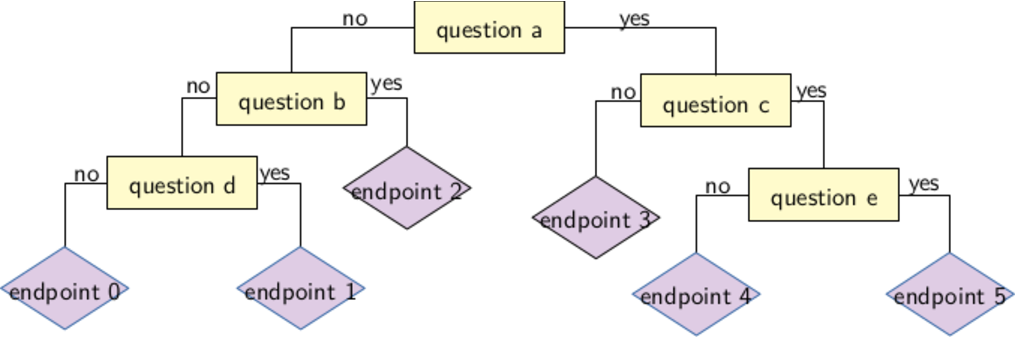
\includegraphics[width=6in]
{dtree/typical-dtree.pdf}
\caption{Typical decision tree.} 
\label{fig-typical-dtree}
\end{figure}

\begin{figure}[h!]
\centering
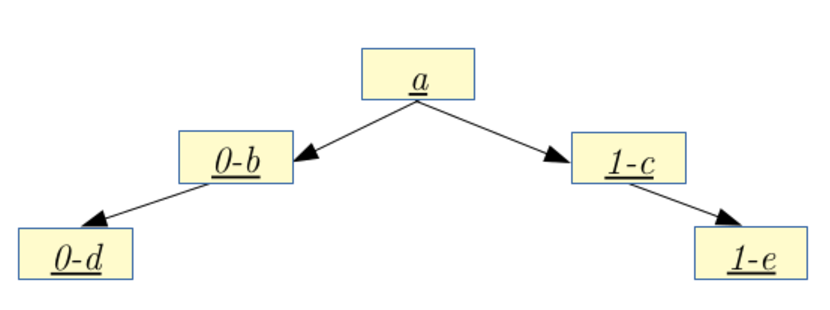
\includegraphics[width=5in]
{dtree/typical-dtree-bnet.pdf}
\caption{Bnet corresponding to 
decision tree
 Fig.\ref{fig-typical-dtree} }
\label{fig-typical-dtree-bnet}
\end{figure}

Fig.\ref{fig-typical-dtree}
shows a typical decision tree (dtree).
The yellow 
rectangles pose 
questions. In general,
the answers to those
questions can
be multiple choices with
more than two choices,
but in Fig.\ref{fig-typical-dtree}
we have chosen the simplest case
of only two choices, 
true or false.
The purple diamonds represent 
endpoints, goals, final
conclusions,
single states of reality, etc.

A trivial 
observation
that is often not made
in dtree educational literature
is that every dtree 
maps into a special bnet, 
let's call it
its ``image" bnet,
in a very simple and natural way.
To get the
 image bnet, just follow the
following simple steps:
\begin{enumerate}
\item {\bf Keep
the yellow question nodes
but reinterpret them as bnet nodes.}
Redraw the connections among
the dtree question nodes
 as arrows pointing
away from the root node.

The image bnet nodes
have 3 states,  $0=no$ and
$1=yes$ and $null$.
Table \ref{tab-ternary-trans-prob}
gives the 
node transition matrix $[P(x|a)]_{
x\in \{0,1,null\}, 
a\in \{0,1,null\}}$
where $p_1\in[0,1]$ can be 
different for each node and is given
in the info that specifies    
the dtree. In Table 
\ref{tab-ternary-trans-prob},
$a_0= 0$ if the
dtree node being replaced has input
``no" and $a_0=1$ if its 
input is ``yes".
$!a_0$ means not $a_0$ (i.e., $!a_0=1-a_0$).
\item
{\bf This method of naming
the image bnet nodes
is not necessary but a good practice.}
Give as names to the image bnet
nodes 
an abridged 
version of
the questions
that label the dtree nodes they replace.
Use as a suffix
to the name of a 
bnet node either a 0 or a 1
depending whether
the dtree node they are replacing
has a 0 or a 1 as input.
This suffix is not
necessary because its
info is already encoded
into
which column
of the node transition matrix has 
zero probability for the
$null$ state, but
it's  a redundancy which makes
the bnet easier to read and understand.
\item {\bf Erase the purple endpoint
nodes and connectors to them.} The
info in the endpoint nodes
can be preserved
by using it
as a more
explicit name
for the output
states of the
leaf node that 
is the parent
to the endpoint 
in the image bnet.
They replace $no=0$ if the
endpoint has 0 as input 
or $yes=1$ if it has 1 as input.
\end{enumerate}

% Please add the following required packages to your document preamble:
% \usepackage[table,xcdraw]{xcolor}
% If you use beamer only pass "xcolor=table" option, i.e. \documentclass[xcolor=table]{beamer}
\begin{table}[h!]
\begin{tabular}{|
>{\columncolor[HTML]{ECF4FF}}l |l|l|l|}
\hline
$P(x|a)$ & \cellcolor[HTML]{ECF4FF}$a=a_0$ & \cellcolor[HTML]{ECF4FF}$a=!a_0$ & \cellcolor[HTML]{ECF4FF}$a=null$ \\ \hline
$x=0$    & $1-p_1$                         & 0                                & 0                                \\ \hline
$x=1$    & $p_1$                           & 0                                & 0                                \\ \hline
$x=null$ & 0                               & 1                                & 1                                \\ \hline
\end{tabular}
\caption{Node transition probability
matrix of a dtree image bnet.}
\label{tab-ternary-trans-prob}
\end{table}

% Please add the following required packages to your document preamble:
% \usepackage[table,xcdraw]{xcolor}
% If you use beamer only pass "xcolor=table" option, i.e. \documentclass[xcolor=table]{beamer}
\begin{table}[h!]
\begin{tabular}{|l|l|}
\hline
\rowcolor[HTML]{ECF4FF} 
\textbf{\begin{tabular}[c]{@{}l@{}}dtree node types\\ (usual shape in parenthesis)\end{tabular}} & \textbf{\begin{tabular}[c]{@{}l@{}}their node transition probability matrix $P(x|a)$\\  in image bnet\end{tabular}}                               \\ \hline
chance node (oval)                                                                               & $P(x|a)$ arbitrary. random                                                                                                                        \\ \hline
decision node (square)                                                                           & \begin{tabular}[c]{@{}l@{}}$P(x|a)=\delta(x, f(a))$\\ where $f(\cdot)$ is a function of $a$. deterministic\end{tabular}                           \\ \hline
endpoint node (diamond)                                                                          & no $P(x|a)$                                                                                                                                       \\ \hline
fixed node                                                                                       & \begin{tabular}[c]{@{}l@{}}$P(x|a)=\delta(x, x_0)$. $x_0$ does not depend on $a$\\ whereas for decision node it does. deterministic.\end{tabular} \\ \hline
\end{tabular}
\caption{dtree node types. }
\end{table}

When drawing dtrees,
some people put
info 
like explanations 
and probabilities on the
connectors 
between the nodes
of  the dtree.
That
info can all
be preserved
in the node names, node state names
and node
transition matrices
of the image bnet nodes.
Often,
the educational literature
states that 
dtrees are more explicit and  
carry
more info than their
image bnets,
but if one 
follows the above
prescriptions,
both can carry
the same info.

A commonly used
deterministic dtree node
is one that 
asks
 the question $x<\alpha?$.
for some 
real number
$\alpha\in (L,U)$ and
 some variable $x$ (for
example, $x=$ height of a person).
For such an interval 
splitting  node,
the transition probability
matrix would be as given
in Fig.\ref{tab-int-split}.
If the interval $[L,U]$
is binned into a number $nbins$
of bins, then
this transition matrix will
have dimensions
 ($nbins +1$,
the number of states of the
parent node).


% Please add the following required packages to your document preamble:
% \usepackage[table,xcdraw]{xcolor}
% If you use beamer only pass "xcolor=table" option, i.e. \documentclass[xcolor=table]{beamer}
\begin{table}[h!]
\begin{tabular}{|
>{\columncolor[HTML]{ECF4FF}}l |l|l|l|}
\hline
$P(x|a)$                                        & \cellcolor[HTML]{ECF4FF}\begin{tabular}[c]{@{}l@{}}states of parent node\\ with $a=a_0$\end{tabular} & \cellcolor[HTML]{ECF4FF}\begin{tabular}[c]{@{}l@{}}states of parent node\\ with $a=!a_0$\end{tabular} & \cellcolor[HTML]{ECF4FF}$a=null$ \\ \hline
$[x\in bin]_{\forall\; bin\subset  [L,\alpha)}$ & 1                                                                                                    & 0                                                                                                     & 0                                \\ \hline
$[x\in bin]_{\forall \;bin\subset  [\alpha,U]}$ & 0                                                                                                    & 0                                                                                                     & 0                                \\ \hline
$x=null$                                        & 0                                                                                                    & 1                                                                                                     & 1                                \\ \hline
\end{tabular}
\caption{Transition probability matrix
for interval splitting node.}
\label{tab-int-split}
\end{table}

A naive Bayes bnet 
(see Chapter \ref{ch-naive})
consists of a single ``class"
 node that fans
out with arrows 
pointing to other
``feature" nodes.
If the leaf nodes
of a naive
Bayes bnet
fan out into 
a set of new leaf
nodes, and those new
leaf nodes
also
fan out
and so on recursively,
we get a 
tree bnet.
The bnet
that arises
from
this recursive
application
of naive Bayes
has the same structure
as the image bnet of a dtree.
However, it is more
general because its node
transition matrices are more general. For
this reason, a recursive
naive Bayes
can be trained to
do more complex classifications.
As a curve fitter, it has more
weights (weight=
parameters of node
transition matrices) than a dtree
with the same graph.



\section*{Influence diagrams and 
their utility nodes}
The bnet literature
often mentions influence
diagrams as a more
general alternative  to dtrees.
{\bf Influence diagrams} are
just arbitrary bnets
enhanced with a 
new kind of node called a {\bf 
utility node}.
The rest
of this section  will 
be devoted to discussing utility nodes.

A utility node
can be
understood
as a node
composed of 3 simpler bnet nodes.
This
is illustrated in Fig.\ref{fig-util-node}.

\begin{figure}[h!]
\centering
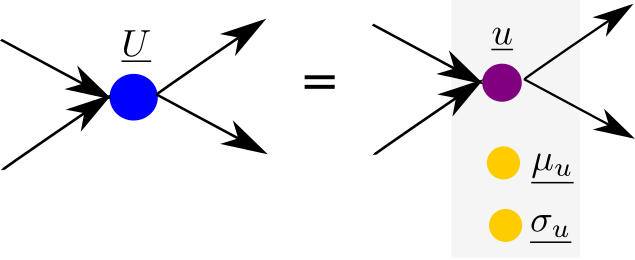
\includegraphics[width=3.5in]
{dtree/util-node.png}
\caption{A utility node
is commonly used in influence
diagrams. It can be
understood
as a node 
composed of 3 simpler bnet nodes.} 
\label{fig-util-node}
\end{figure}

The transition probability matrices,
printed in blue,
for the nodes
of Fig.\ref{fig-util-node},
are as follows:

\beq\color{blue}
P(U|pa(U))\text{ = given}
\eeq

\beq\color{blue}
P(u|pa(U))=
P(U=u|pa(U))
\eeq

Node $\ul{\mu}_u$
calculates the
expected value (mean value) of $\rvu$:

\beq\color{blue}
P(\mu_u)=\delta(\mu_u,
E_{\rvu}[\rvu])
\eeq

Node $\ul{\sigma}_u$
calculates the
standard deviation of $\rvu$:
\beq\color{blue}
P(\sigma_u)=\delta(\sigma_U,
\sqrt{
E_{\rvu}[
(u-E_{\rvu}[\rvu])^2]})
\eeq

Note that in order to
calculate expected values,
it is necessary that
$\rvU, \rvu\in \RR$. Note that
nodes $\rvu$, $\ul{\mu}_u$, $\ul{\sigma}_u$
must all 3 have access
to the 
transition matrix
$P(U|pa(U))$ of node $\rvU$.
In fact, in order  to
calculate $E_\rvu[\cdot]$,
it is necessary for
nodes $\ul{\mu}_u$ and 
 $\ul{\sigma}_u$
to have access not just to 
$P(U|pa(U))$ but also to
$P(pa(U))$.

See Fig.\ref{fig-util-merge}.
An influence
diagram may have multiple
utility nodes ($\rvU_1$ and
$\rvU_2$ in Fig.\ref{fig-util-merge}).
Then one can define a merger
utility node $\rvU$ that adds
all the other utility 
nodes.

\begin{figure}[h!]
\centering
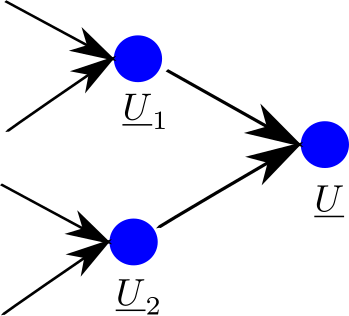
\includegraphics[width=1.5in]
{dtree/util-merge.png}
\caption{An influence
diagram may have multiple
utility nodes, say $\rvU_1$ and
$\rvU_2$. Then
one can define a
utility node $\rvU=\rvU_1 + \rvU_2$. } 
\label{fig-util-merge}
\end{figure}

\beq\color{blue}
P(U|U_1, U_2)=\delta(U,
U_1 + U_2)
\eeq